\documentclass[]{article}
\newcommand{\FileDepth}{../..}
\usepackage[a4paper, total={15cm,23cm}]{geometry}
\usepackage[T1]{fontenc}
\usepackage{textcomp}%Not strictly necessary, but gives \textmu command for "micro."
\usepackage{fancyhdr}
\usepackage{amsmath}
\usepackage{amssymb}
\usepackage{graphicx}
\usepackage{xcolor}
\usepackage{tikz}
\usetikzlibrary{calc}
%opening
\newcommand{\SecType}{X}
\newcommand{\Week}{X}
\title{Representations of Volume}
\author{Benjamin Bauml}
\date{Summer 2024}
\pagestyle{fancy}
\rhead{PH 211}
\chead{Summer 2024}
\lhead{Week \Week}

% For Assignment, leave Purpose as 1. For Worksheet, set to 2. For Student Solution, set to 3. For Teacher Solution, set to 4.
% If you want keep the pieces from being called manually, set DefOnly to 0.
\newcommand{\Purpose}{4}
\newcommand{\DefOnly}{1}

% Version 2024-04-27
% Changes
% 2024-02-21 Added xstring package to enable smooth implementation of new \ModePage command.
% 2024-04-27 Set up to split activities and formatting aspects into separate files. Removed dependence on xcomment. Added an automatic counter to number the activities in a problem set.
% 2024-05-19 Revised old format for \TeachingTips command, which did not support \DefOnly.
\usepackage{tcolorbox}
\usepackage{xstring}
% You will want the following four lines in your document (the last two uncommented):
% For Assignment, leave Purpose as 1. For Worksheet, set to 2. For Student Solution, set to 3. For Teacher Solution, set to 4.
% If you want keep the pieces from being called manually, set DefOnly to 0.
%\newcommand{\Purpose}{4}
%\newcommand{\DefOnly}{1}
\newcommand{\Exclusion}{0}
\newcommand{\PageTurn}{0}
\newcommand{\GrayProb}{0}
\newcommand{\Tipsy}{0}

% Assignment
\if\Purpose1
\renewcommand{\Exclusion}{1}
\fi
% Worksheet
\if\Purpose2
\renewcommand{\Exclusion}{1}
\renewcommand{\PageTurn}{1}
\fi
% Student Solution
\if\Purpose3
\renewcommand{\PageTurn}{1}
\renewcommand{\GrayProb}{1}
\fi
% Teaching Copy
\if\Purpose4
\renewcommand{\PageTurn}{1}
\renewcommand{\GrayProb}{1}
\renewcommand{\Tipsy}{1}
\fi

\def \NewQ {0}
\def \PForce {0}
\newcommand{\MaybePage}[1]{
	\def \PForce {#1}
	\if\PForce1
	\newpage
	\else
	\if\NewQ0
	\gdef \NewQ {\PageTurn}
	\else
	\newpage
	\fi
	\fi
}

\newcommand{\ModePage}[1]{
	\IfSubStr{#1}{\Purpose}{\newpage}{}
}

\newcounter{ActNumber}
\setcounter{ActNumber}{0}

\newcommand{\Problem}[4][0]{%The first argument is optional, and if it is set to 1, the \newpage will be forced. The second argument is the name of the activity, the third is the command the activity is stored as, and the fourth is the actual problem statement.
\newcommand{#3}{
\MaybePage{#1}
\addtocounter{ActNumber}{1}
\section*{\SecType\Week-\theActNumber: #2}
\if\GrayProb1
\begin{tcolorbox}[colback=lightgray,colframe=lightgray,sharp corners,boxsep=1pt,left=0pt,right=0pt,top=0pt,bottom=0pt,after skip=2pt]
\else
\begin{tcolorbox}[colback=white,colframe=white,sharp corners,boxsep=1pt,left=0pt,right=0pt,top=0pt,bottom=0pt,after skip=2pt]
\fi
#4
\end{tcolorbox}\noindent
}
\if\DefOnly0
\else
#3
\fi
}
	
\newcommand{\ProblemSub}[3][0]{%The first argument is optional, and if a string of numbers is entered into it, it will force a \newpage in any \Purpose that shows up in the string. For example, "13" would lead to the newpage being forced in modes 1 and 3. The second is the command the activity is stored as, and the third is the actual problem statement.
\newcommand{#2}{
\ModePage{#1}
\if\GrayProb1
\begin{tcolorbox}[colback=lightgray,colframe=lightgray,sharp corners,boxsep=1pt,left=0pt,right=0pt,top=0pt,bottom=0pt,after skip=2pt]
\else
\begin{tcolorbox}[colback=white,colframe=white,sharp corners,boxsep=1pt,left=0pt,right=0pt,top=0pt,bottom=0pt,after skip=2pt]
\fi
#3
\end{tcolorbox}\noindent
}
\if\DefOnly0
\else
#2
\fi
}
		
\newcommand{\Solution}[2]{%The first argument is the command the solution is stored as, and the second is the actual solution.
\newcommand{#1}{
\if\Exclusion0
#2
\fi
}
\if\DefOnly0
\else
#1
\fi
}
		
\newcommand{\ProblemFig}[2]{%The first argument is the command the figure is stored as, and the second is the actual figure.
\newcommand{#1}{
\begin{figure}[h]
#2
\end{figure}
}
\if\DefOnly0
\else
#1
\fi
}

\newcommand{\TeachingTips}[2]{%The first argument is the command the tip is stored as, and the second is the actual tip.
\newcommand{#1}{
\if\Tipsy1
\begin{tcolorbox}[colback=lightgray,colframe=black]
#2
\end{tcolorbox}
\fi
}
\if\DefOnly0
\else
#1
\fi
}

%\newcommand{\FBDaxes}[3]{
	\begin{scope}[shift={(#1)},rotate=#2]
		% x-axis
		\draw[thick,->] (-2,0) -- (2,0);
		\node[anchor=west] at (2,0) {$x$};
		% y-axis
		\draw[thick,->] (0,-2) -- (0,2);
		\node[anchor=west] at (0,2) {$y$};
		\coordinate (#3) at (0,0);
	\end{scope}
}
\newcommand{\FBDvectorMA}[4]{
	\begin{scope}[shift={(#1)}]
		\coordinate (#4tip) at ({#2*cos(#3)},{#2*sin(#3)});
		\draw[ultra thick,blue,->] (#1) -- (#4tip);
	\end{scope}
}
\newcommand{\FBDvectorXY}[3]{
	\begin{scope}[shift={(#1)}]
		\coordinate (#3tip) at (#2);
		\draw[ultra thick,blue,->] (0,0) -- (#3tip);
	\end{scope}
}
\newcommand{\FBDdot}[1]{
	\filldraw[black] (#1) circle (3pt);
}
%\newcommand{\MVec}[3][0]{%Creates a momentum vector of length #3 centered at #2 and rotated #1 degrees counterclockwise.
	\begin{scope}[rotate=#1,shift={(#2)}]
		\draw[->,thick] ({-#3/2},0) -- ({#3/2},0);
	\end{scope}
}
\newcommand{\MDot}[1]{%Creates a dot at #1 to represent a zero vector.
	\filldraw (#1) circle (1pt);
}
\newcommand{\MVDRows}[2][4.5]{%Creates the rows (initial, delta, final) of a momentum vector diagram. The optional argument determines the width of the table, and defaults to a good length for three columns (two objects and the total system). The non-optional argument gives a coordinate name (not displayed) to the diagram.
	\begin{scope}
		%\draw[thick] (0,5.5) -- (0,0);
		\draw[thick] (-1,4.5) -- (#1,4.5);
		\node at (-0.5,3.75) {$\vec{p}_{i}$};
		\draw[thick] (-1,3) -- (#1,3);
		\node at (-0.5,2.25) {$\Delta\vec{p}$};
		\draw[thick] (-1,1.5) -- (#1,1.5);
		\node at (-0.5,0.75) {$\vec{p}_{f}$};
		\coordinate (#2) at (0,5);
	\end{scope}
}
\newcommand{\MVDCol}[4][0.75]{%Creates a column for an object in a momentum vector diagram. The first (non-optional) argument is the coordinate name (not displayed) of the column, while the second is the displayed column header. The first argument also names the three entries down the column. The third argument anchors the column, so it should either be the coordinate name of the MVD (for the first column) or the coordinate name of the previous column. The optional argument indicates how far the center of the column should be from the previous column's edge, and defaults to 0.75
	\begin{scope}[shift={(#4)}]
		\node at (#1,0) {#3};
		%\draw[thick] ({#1*2},0.5) -- ({#1*2},-5);
		\draw[thick] (0,0.5) -- (0,-5);
		\coordinate (#2init) at (#1,-1.25);
		\coordinate (#2delt) at (#1,-2.75);
		\coordinate (#2fin) at (#1,-4.25);
		\coordinate (#2) at ({#1*2},0);
	\end{scope}
}

\begin{document}
\maketitle

\Problem{Representations of Volume}{\VolReps}{
You want to determine the volume of the room you are in.
}
\ProblemSub{\VolRepsA}{
(a) Write a description of how to find the volume of the room in words.
}
\Solution{\VolRepsASol}{

If we measure the dimensions of the room (ceiling height, length, width), and multiply them together, we can get a decent estimate of the volume of the room.

Of course, it won't be perfect. The floor isn't even, the walls have a few pillars embedded in them, the doors lie in slight recesses, and there are air ducts sticking into the room. We could find their volumes and subtract, perhaps, if we need that level of accuracy.

Instead, we will assume for simplicity that the room is rectangular and empty.
}
\ProblemSub{\VolRepsB}{
(b) Sketch a diagram that would help you find the volume of the room.
}
\Solution{\VolRepsBSol}{

\begin{figure}[h]
	\centering
	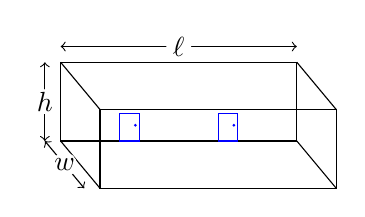
\begin{tikzpicture}
		\begin{scope}
			\coordinate (nearll) at (0,0);
			\coordinate (nearlr) at (3,0);
			\coordinate (nearur) at (3,1);
			\coordinate (nearul) at (0,1);
			\draw (nearll) -- (nearlr) -- (nearur) -- (nearul) -- cycle;
		\end{scope}
		\begin{scope}[shift={(-0.5,0.6)}]
			\coordinate (farll) at (0,0);
			\coordinate (farlr) at (3,0);
			\coordinate (farur) at (3,1);
			\coordinate (farul) at (0,1);
			\draw (farll) -- (farlr) -- (farur) -- (farul) -- cycle;
			\draw[<->] (0,1.2) -- (3,1.2);
			\filldraw[white] (1.5,1.2) circle (0.15);
			\node at (1.5,1.2) {$\ell$};
			\draw[<->] (-0.2,0) -- (-0.2,1);
			\filldraw[white] (-0.2,0.5) circle (0.15);
			\node at (-0.2,0.5) {$h$};
			\begin{scope}[shift={(0.75,0)}]
				\draw[blue] (0,0) -- (0.25,0) -- (0.25,0.35) -- (0,0.35) -- cycle;
				\draw[blue] (0.2,0.2) circle (0.01);
			\end{scope}
			\begin{scope}[shift={(2,0)}]
				\draw[blue] (0,0) -- (0.25,0) -- (0.25,0.35) -- (0,0.35) -- cycle;
				\draw[blue] (0.2,0.2) circle (0.01);
			\end{scope}
		\end{scope}
		\draw (nearll) -- (farll);
		\draw (nearlr) -- (farlr);
		\draw (nearur) -- (farur);
		\draw (nearul) -- (farul);
		\draw[<->] (-0.2,0) -- (-0.7,0.6);
		\filldraw[white] (-0.45,0.3) circle (0.15);
		\node at (-0.45,0.3) {$w$};
	\end{tikzpicture}
\end{figure}

I put the {\color{blue}doors} in to orient the drawing. They are otherwise not critical, and their sizes and positions are not quantitatively accurate.
}
\ProblemSub{\VolRepsC}{
(c) Write a symbolic expression that would allow you to find the volume of the room. Check the units of your expression.
}
\Solution{\VolRepsCSol}{

\[
V = \ell w h
\]
Length $\ell$, width $w$, and height $h$ are all lengths, which would be measured in meters in SI units. Volume is measured in m$^{3}$ in SI units. When we multiply $\ell w h$, we are multiplying meters by meters by meters, which gives us m$^{3}$, so we have the same units on either side of the equal sign:
\[
[V] = \text{m}^{3}, \qquad [\ell w h] = [\ell][w][h]=\text{m}\cdot\text{m}\cdot\text{m}=\text{m}^{3}.
\]
}
\ProblemSub{\VolRepsD}{
(d) Without standing up, estimate the volume of the room as a number. Make sense of the number by comparing it to something.
}
\Solution{\VolRepsDSol}{

There are several ways to estimate the dimensions of the room without measuring it directly:
\begin{itemize}
	\item Guess your local TA's height (or just ask) and compare them to the height of the ceiling, like a living measuring stick.
	\item Look up the height of a standard interior door (Home Depot says 80 inches, which is about 2.032 meters) and estimate how many doors high the ceiling is.
	\item The carpet tiles are a regular size. Measure one nearby and count how many you see from one wall to another.
\end{itemize}
For comparison, an Olympic pool is about 2500 m$^{3}$ (technically, there is no standard depth, so this can vary). Comparing this to the size of the room can give you some idea about how accurate your estimate is (for example, the room is certainly not larger than an Olympic pool).
}
\end{document}